\chapter{User Interface Design}

Different mock-ups of the application have been shown in the \gls{rasd}.
In the current document we are going to present the \gls{ux} diagram~\ref{fig:UXDiagram} to help the reader in the understanding of the sequence of events and the relations between interfaces.

\begin{figure}[H]
    \centering
    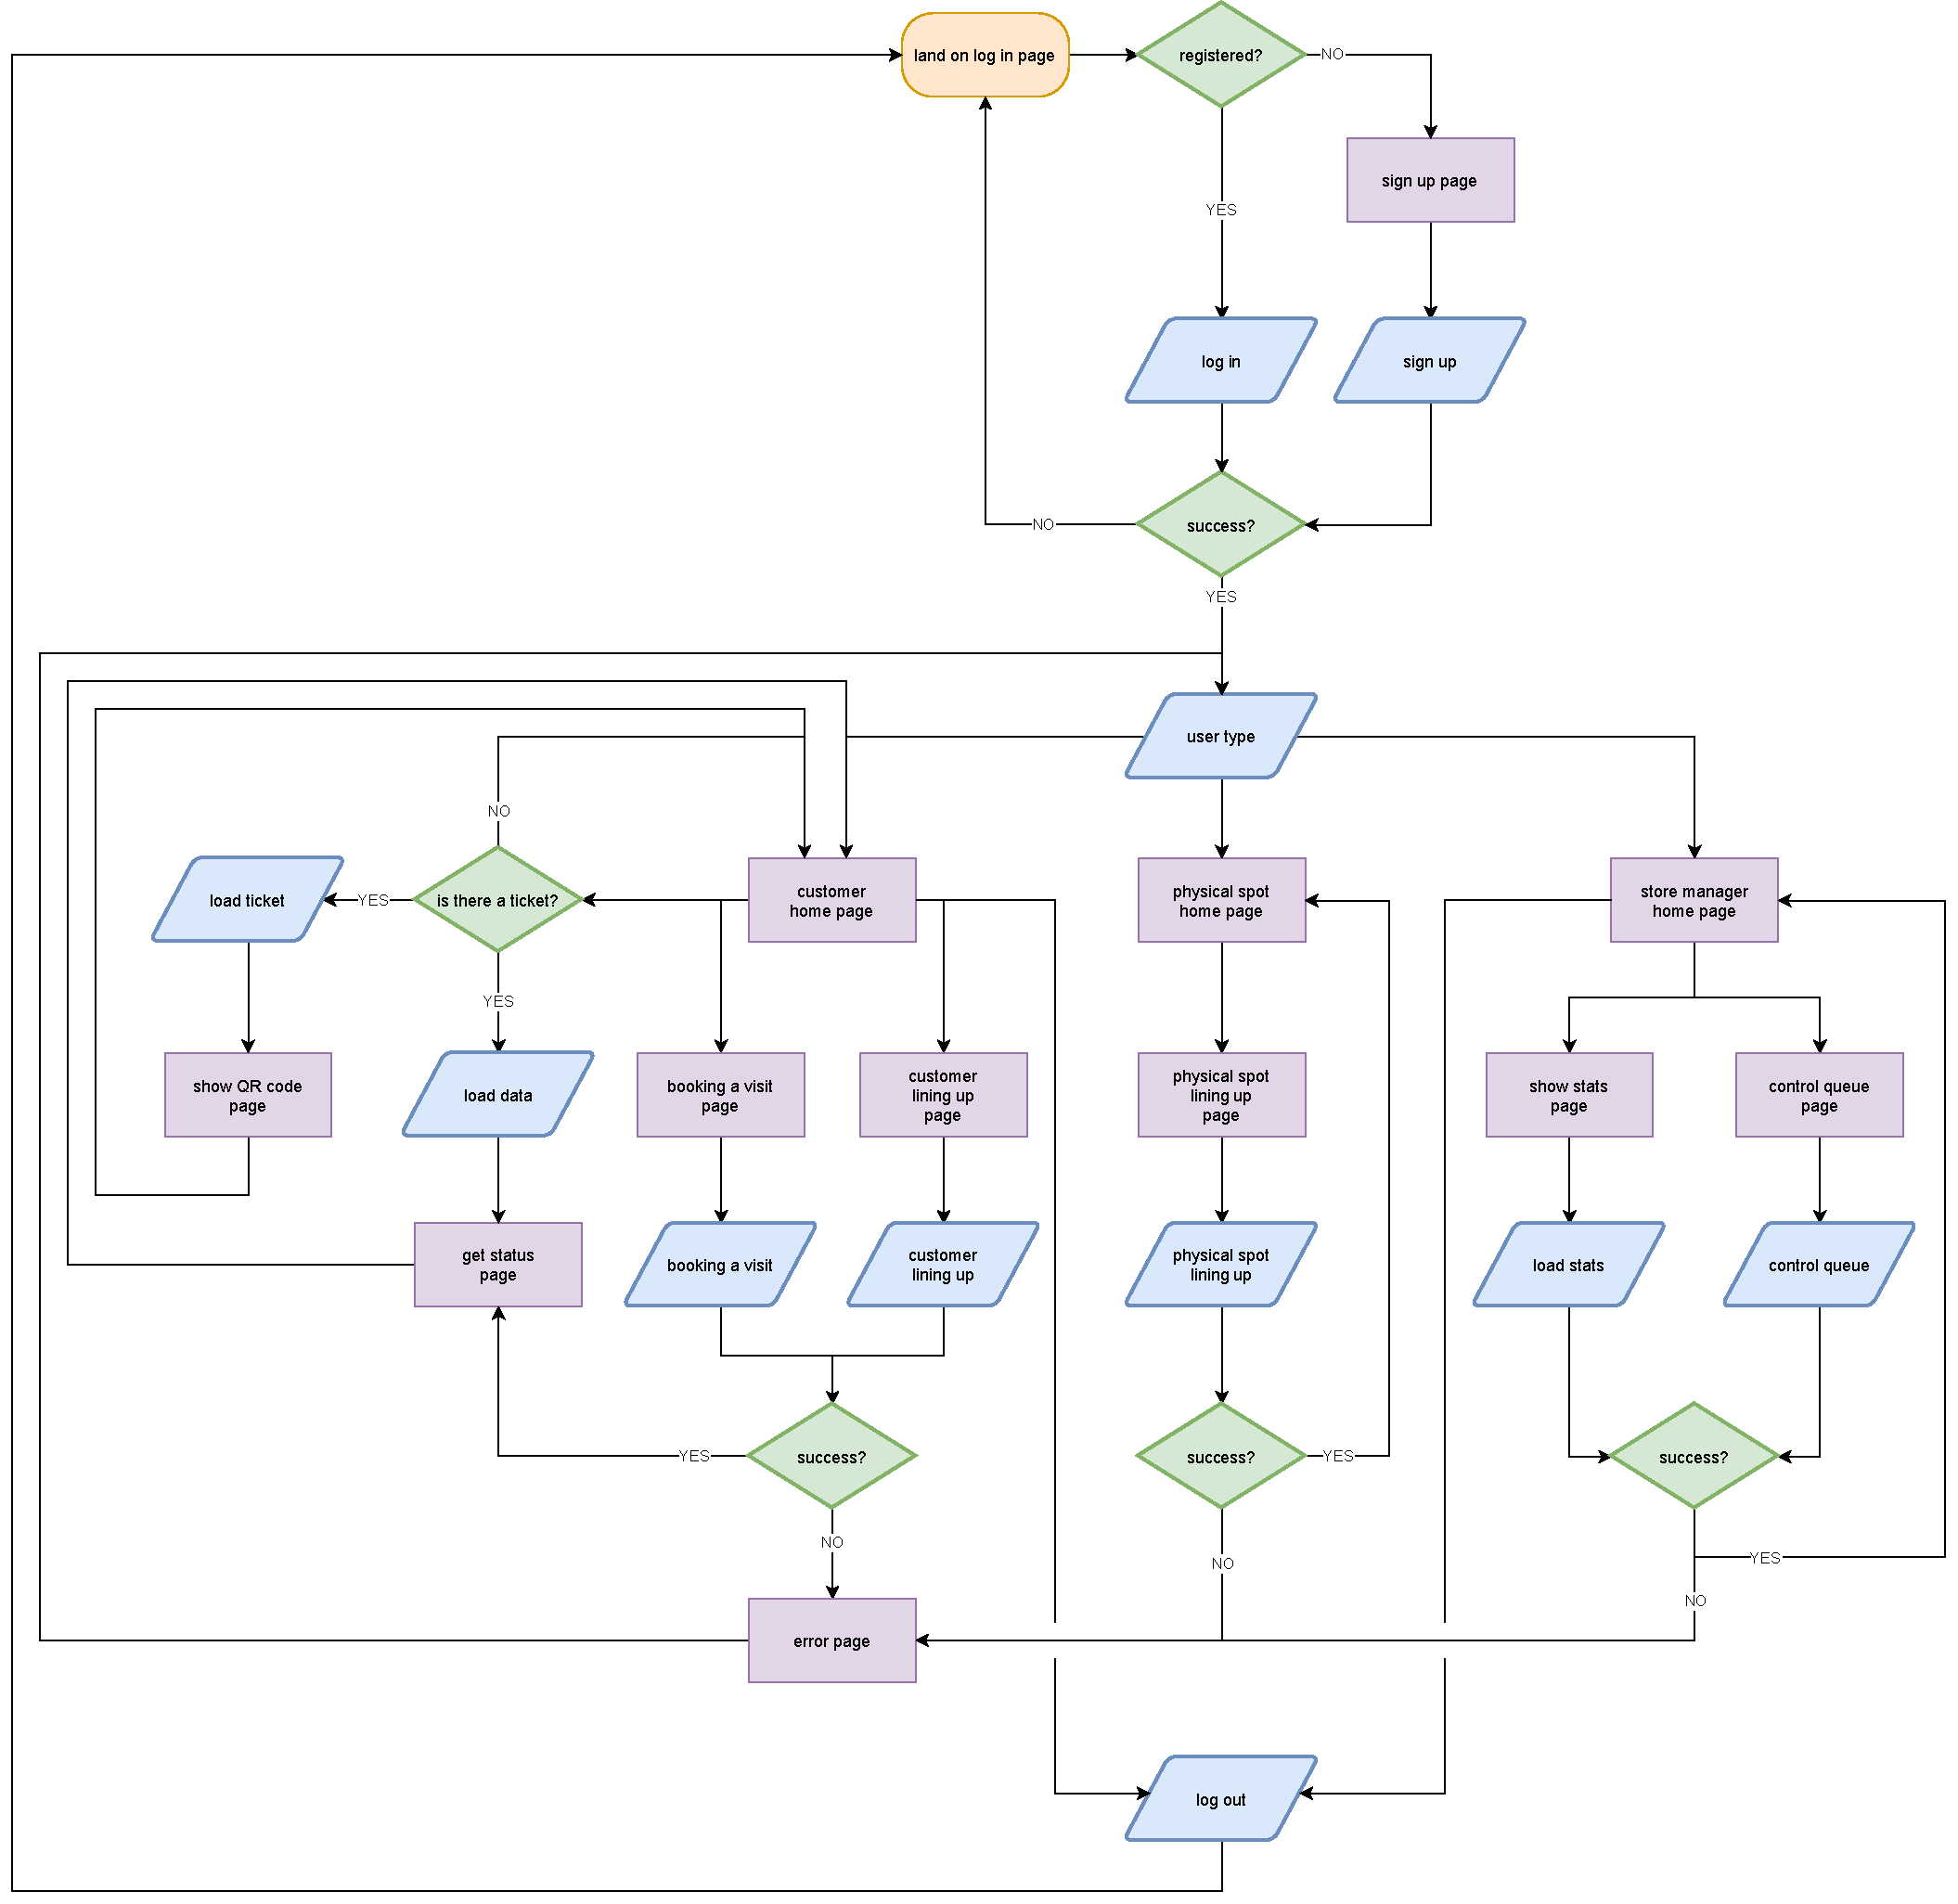
\includegraphics[width=0.9\textwidth]{images/UX.pdf}
    \caption{\gls{ux} diagram. \textit{Yellow} boxes represent \textbf{start}ing and \textbf{end}ing \textbf{points}. \textit{Green} boxes are for \textbf{decisions}. \textit{Violet} boxes are for \textbf{processes}. \textit{Blue} boxes are for \textbf{inputs/outputs}.}\label{fig:UXDiagram}
\end{figure}

